\chapter{NVARs in Practice}\label{ch:nvar-application}

\section{State Inference with Lorenz '63}

\begin{figure}
  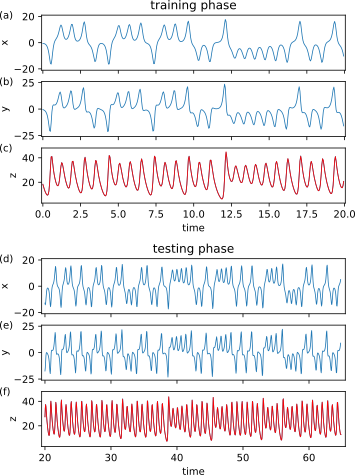
\includegraphics{figures/nvar-infer-lorenz}
  \caption{FIXME caption.}
  \label{fig:nvar-infer-lorenz}
\end{figure}

\section{Forecasting Lorenz '63}

\begin{figure}
  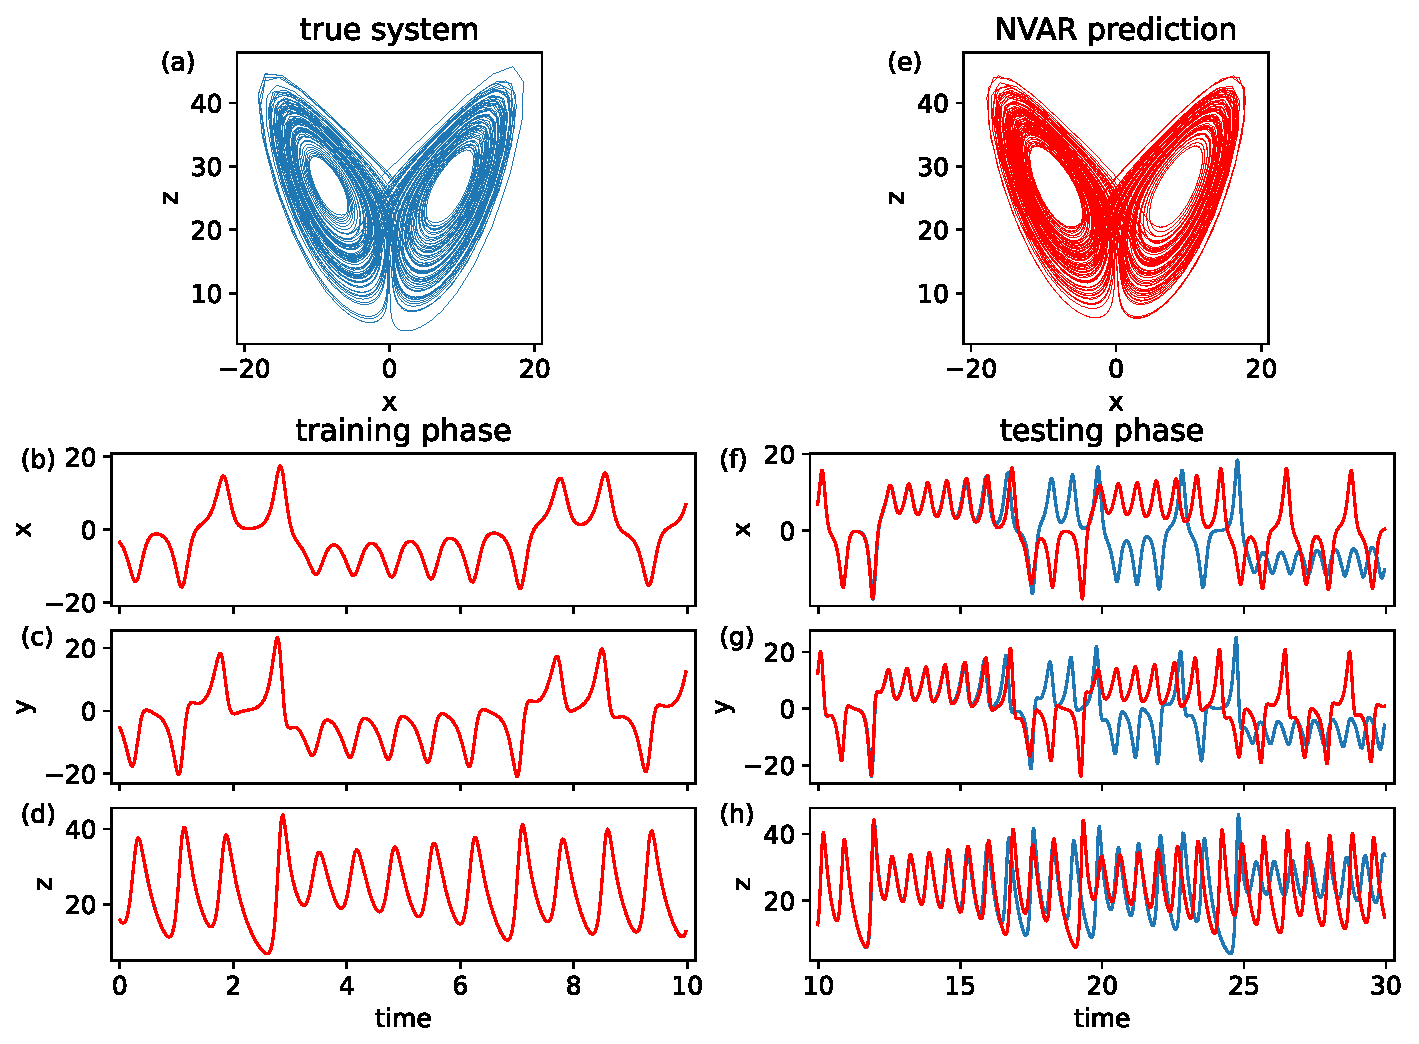
\includegraphics[width=\textwidth]{figures/nvar-predict-lorenz}
  \caption{FIXME caption.}
  \label{fig:nvar-predict-lorenz}
\end{figure}

\begin{figure}
  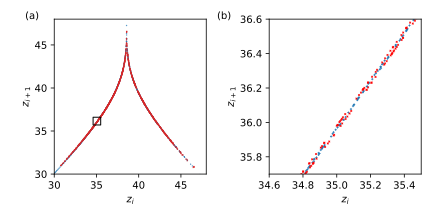
\includegraphics{figures/nvar-lorenz-rmap}
  \caption{FIXME caption.}
  \label{fig:nvar-lorenz-rmap}
\end{figure}

\begin{figure}
  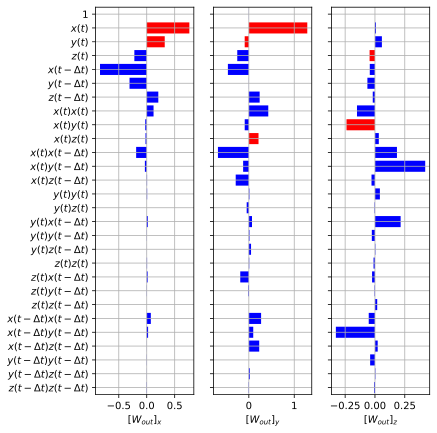
\includegraphics{figures/nvar-predict-lorenz-wout}
  \caption{FIXME caption.}
  \label{fig:nvar-predict-lorenz-wout}
\end{figure}

\section{Forecasting the Double-Scroll Circuit}

\begin{figure}
  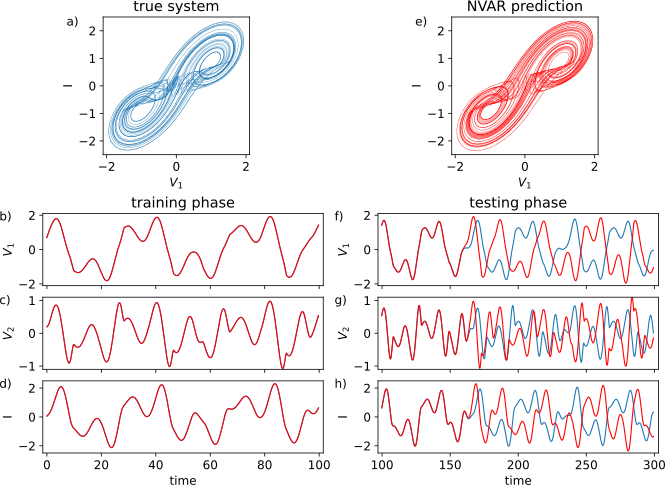
\includegraphics[width=\textwidth]{figures/nvar-predict-dscroll}
  \caption{FIXME caption.}
  \label{fig:nvar-predict-dscroll}
\end{figure}

\section{Forecasting Mackey-Glass}

\begin{figure}
  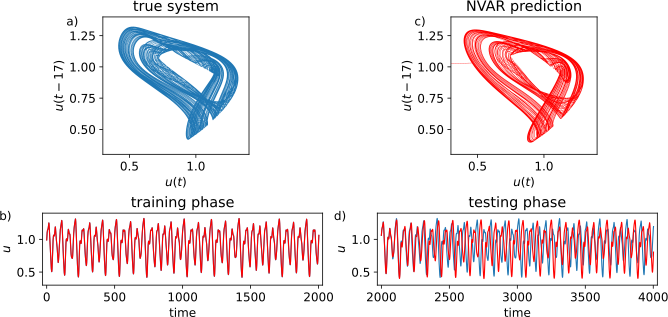
\includegraphics[width=\textwidth]{figures/nvar-predict-mackey-glass}
  \caption{FIXME caption.}
  \label{fig:nvar-predict-mackey-glass}
\end{figure}
